\begin{figure}[ht]
    \centering
    \begin{subfigure}[b]{0.45\textwidth}
        \includegraphics[width=\textwidth]{img/inpainting/rof/006lena.png}
        \caption{$\lambda = 0.06$}
    \end{subfigure}
    \begin{subfigure}[b]{0.45\textwidth}
        \includegraphics[width=\textwidth]{img/inpainting/rof/007lena.png}
        \caption{$\lambda = 0.07$}
    \end{subfigure}
    \begin{subfigure}[b]{0.45\textwidth}
        \includegraphics[width=\textwidth]{img/inpainting/rof/009lena.png}
        \caption{$\lambda = 0.09$}
    \end{subfigure}
    \begin{subfigure}[b]{0.45\textwidth}
        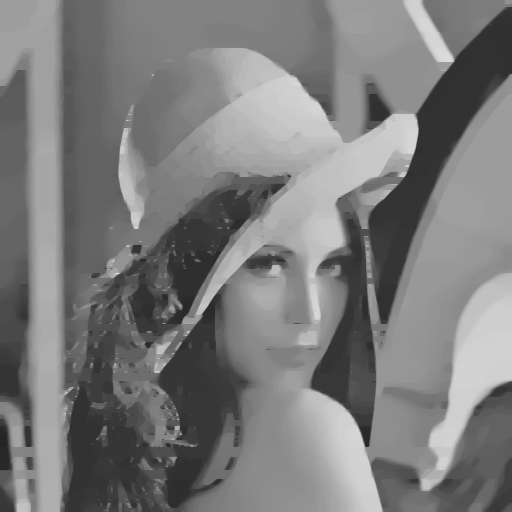
\includegraphics[width=\textwidth]{img/inpainting/rof/01lena.png}
        \caption{$\lambda = 0.1$}
    \end{subfigure}
    \caption{Inpainting of Lena image with the ROF Model.}
\label{fig:inpainting_lena_rof}
\end{figure}